%----------------------------------------------------------------------------------------
%	PACKAGES AND OTHER DOCUMENT CONFIGURATIONS
%----------------------------------------------------------------------------------------

\documentclass[11pt]{scrartcl} % Font size

%%%%%%%%%%%%%%%%%%%%%%%%%%%%%%%%%%%%%%%%%
% Wenneker Assignment
% Structure Specification File
% Version 2.0 (12/1/2019)
%
% This template originates from:
% http://www.LaTeXTemplates.com
%
% Authors:
% Vel (vel@LaTeXTemplates.com)
% Frits Wenneker
%
% License:
% CC BY-NC-SA 3.0 (http://creativecommons.org/licenses/by-nc-sa/3.0/)
% 
%%%%%%%%%%%%%%%%%%%%%%%%%%%%%%%%%%%%%%%%%

%----------------------------------------------------------------------------------------
%	PACKAGES AND OTHER DOCUMENT CONFIGURATIONS
%----------------------------------------------------------------------------------------

\usepackage{amsmath, amsfonts, amsthm} % Math packages

\usepackage{listings} % Code listings, with syntax highlighting

\usepackage{graphicx} % Required for inserting images

\usepackage{booktabs} % Required for better horizontal rules in tables

\usepackage{dirtytalk} % Required for quoting.

\usepackage{float} % Added for hard placement of images.

\usepackage[dvipsnames]{xcolor} % Added for extra colors.

\usepackage{tikz} % For colored boxes and more.

\numberwithin{equation}{section} % Number equations within sections (i.e. 1.1, 1.2, 2.1, 2.2 instead of 1, 2, 3, 4)
\numberwithin{figure}{section} % Number figures within sections (i.e. 1.1, 1.2, 2.1, 2.2 instead of 1, 2, 3, 4)
\numberwithin{table}{section} % Number tables within sections (i.e. 1.1, 1.2, 2.1, 2.2 instead of 1, 2, 3, 4)

\usepackage{enumitem} % Required for list customisation
\setlist{noitemsep} % No spacing between list items

\usepackage[main=greek, english]{babel}

%----------------------------------------------------------------------------------------
%	DOCUMENT MARGINS
%----------------------------------------------------------------------------------------

\usepackage{geometry} % Required for adjusting page dimensions and margins

\geometry{
	paper=a4paper, % Paper size, change to letterpaper for US letter size
	top=2.5cm, % Top margin
	bottom=3cm, % Bottom margin
	left=3cm, % Left margin
	right=3cm, % Right margin
	headheight=0.75cm, % Header height
	footskip=1.5cm, % Space from the bottom margin to the baseline of the footer
	headsep=0.75cm, % Space from the top margin to the baseline of the header
	%showframe, % Uncomment to show how the type block is set on the page
}

%----------------------------------------------------------------------------------------
%	FONTS
%----------------------------------------------------------------------------------------

\usepackage[utf8]{inputenc} % Required for inputting international characters
\usepackage[T1]{fontenc} % Output font encoding for international characters

\usepackage{XCharter} % Use the XCharter fonts


%----------------------------------------------------------------------------------------
%	SECTION TITLES
%----------------------------------------------------------------------------------------

\usepackage{sectsty} % Allows customising section commands

\sectionfont{\vspace{6pt}\centering\normalfont\scshape} % \section{} styling
\subsectionfont{\normalfont\bfseries} % \subsection{} styling
\subsubsectionfont{\normalfont\itshape} % \subsubsection{} styling
\paragraphfont{\normalfont\scshape} % \paragraph{} styling

%----------------------------------------------------------------------------------------
%	HEADERS AND FOOTERS
%----------------------------------------------------------------------------------------

\usepackage{scrlayer-scrpage} % Required for customising headers and footers

\ohead*{} % Right header
\ihead*{} % Left header
\chead*{} % Centre header

\ofoot*{} % Right footer
\ifoot*{} % Left footer
\cfoot*{\pagemark} % Centre footer

\newcommand{\img}[1] % maybe add a caption to this
{
    \begin{center}
        \fcolorbox{black}{white}{\includegraphics[width=\textwidth]{#1}}
    \end{center}

}

% Helper Macros

\newcommand{\en}[1]{\foreignlanguage{english}{#1}}
\newcommand{\src}[1]{{\texttt{#1}}}


% Extra Formatting

\setlength{\parindent}{0em}
\setlength{\parskip}{0em}


% Code Listing Style

\lstdefinestyle{code}{
  belowcaptionskip=1\baselineskip,
  breaklines=true,
  frame=LRTB,
  xleftmargin=\parindent,
  showstringspaces=false,
  basicstyle=\ttfamily,
  keywordstyle=\bfseries\color{green!40!black},
  commentstyle=\itshape\color{purple!40!black},
  identifierstyle=\color{black},
  stringstyle=\color{orange},
}


\newcommand{\lstcode}[3]
{
    \begin{otherlanguage}{english}
    \lstinputlisting[language=#2, frame=single, style=code, caption=#3]{#1}
    \end{otherlanguage}
}
 % Include the file specifying the document structure and custom commands

%----------------------------------------------------------------------------------------
%	TITLE SECTION
%----------------------------------------------------------------------------------------

\title{	
	\normalfont\normalsize
	\textsc{Πανεπιστήμιο Πατρών, Τμήμα Μηχανικών ΗΥ και Πληροφορικής}\\ % Your university, school and/or department name(s)
	\vspace{25pt} % Whitespace
	\rule{\linewidth}{0.5pt}\\ % Thin top horizontal rule
	\vspace{20pt} % Whitespace
	{\LARGE Λογισμικό και Προγραμματισμός Συστημάτων Υψηλής Επίδοσης\\ Άσκηση 1 - MPI και ΜΔΕ}\\ % The assignment title
	\vspace{12pt} % Whitespace
	\rule{\linewidth}{2pt}\\ % Thick bottom horizontal rule
	\vspace{12pt} % Whitespace
}


\author{Ευάγγελος Λάμπρου \and Ιωάννης Παναρίτης} % Your name

\date{} % Today's date (\today) or a custom date

%----------------------------------------------------------------------------------------
%	DOCUMENT
%----------------------------------------------------------------------------------------

\bibliographystyle{abbrv}
\addto\captionsgreek{\renewcommand{\refname}{Αναφορές}}

\begin{document}

\maketitle 

\section{2D Diffusion και MPI}

    \subsection{Υλοποίηση}
        Επιλέχθηκε το blocking implementation για την υλοποίησή.\\
        Πραγματοποιήθηκε αλλαγή στις συναρτήσεις \src{init(), initialize\_density(), advance(),\\compute\_diagnostics()}.

        Για την επικοινωνία μεταξύ των διεργασιών χωρίζουμε ολόκληρο το grid σε τετράγωνα, με την κάθε διεργασία να χειρίζεται ένα από αυτά.
        Η επικοινωνία μεταξύ των διεργασιών γίνεται με την ανταλλαγή των γειτονικών στηλών και γραμμών. \cite{ghostcellpattern}

        \begin{figure}[htpb]
            \centering
            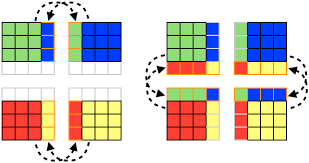
\includegraphics[width=0.5\textwidth]{./assets/ghostcells.png}
            \caption{Η ανταλλαγή ghost cell στηλών και γραμμών μεταξύ των διεργασιών.}
        \end{figure}
        
        \subsubsection*{Αρχικές μετατροπές}
            Προσθέτουμε στο \src{struct Diffusion2D}:
            \begin{itemize}
                \item \src{Local\_N, Square\_N} ώστε να γνωρίζουμε το μέγεθος του κάθε τετραγώνου
                \item Buffer για send, receive με τους γείτονές του.
            \end{itemize}
            
        \subsubsection*{\src{Init()}}
            \begin{itemize}
                 \item Υπολογισμός \src{grid\_size}, για να ξέρουμε σε πόσα μέλη χωρίζεται η κάθε πλευρά.
                \item Υπολογισμός του \src{square\_N} και των υπολοιπών τιμών που χρειαζόμαστε.
                \item Δέσμευση χώρου για \src{right, left} ανταλλαγή δεδομένων.
            \end{itemize}
        \subsubsection*{\src{Initialize\_density()}}
            \begin{itemize}
                \item Χρήση \src{Local\_N\_} αντί για \src{N\_}
                \item Υπολογισμός \src{gj} και χρήση του αντί για \src{j}
            \end{itemize}
        \subsubsection*{\src{Advance()}}
            \begin{itemize}
                \item Χρήση \src{Local\_N\_} αντί για \src{N\_}
                \item Υπολογισμός \src{id} των γειτόνων \src{(left, right, up, down)}
                \item Send και Receive δεδομένων με τους γείτονες
            \end{itemize}
        \subsubsection*{\src{compute\_diagnostics()}}
        \begin{itemize}
            \item Χρήση \src{Local\_N\_} αντί για \src{N\_}
        \end{itemize}

    \subsection{Μετρήσεις}

    Οι μετρήσεις έγιναν σε σύστημα με χαρακτηριστικά: 

    \begin{itemize}
        \item Processor: AMD Ryzen 7 2700 Eight-Core Processor 3.20 GHz
        \item RAM: 16.0 GB
        \item Operating System: 64-bit Linux
    \end{itemize}
    
    \centering
    \begin{tabular}{|p{3cm}||p{3cm}|p{3cm}|}
        \hline
        \multicolumn{3}{|c|}{Execution Time ($s$)} \\
        \hline
        \src{N} & 1 process & 4 processes\\
        \hline
        1024 & 1.677881 & 0.741665\\
        2048 & 6.756217 & 4.03658\\
        4096 & 26.015809 & 15.681488\\
        \hline
    \end{tabular}
        
\section{Chekpointing με MPI I/O}
    Υλοποίηση συναρτήσεων \src{write\_density\_mpi()} και \src{read\_density\_mpi()}
    \subsubsection*{\src{write\_density\_mpi()}}
        \begin{itemize}
            \item Άνοιγμα αρχείου για \src{write}
            \item Υπολογισμός \src{length} και \src{offset}
            \item \src{rho\_tmp $\leftarrow $ rho}
            \item Αποθήκευση του πίνακα \src{rho\_tmp} στο αρχείο, αρχίζοντας από \src{offset} για \src{len doubles} 
        \end{itemize}
    \subsubsection*{\src{read\_density\_mpi()}}
        \begin{itemize}
            \item Άνοιγμα αρχείου για \src{read}
            \item Υπολογισμός \src{length} και \src{offset}
            \item Δίαβασμα \src{len doubles} από \src{offset} και αποθήκευση στο \src{rho\_tmp}
            \item \src{rho $\leftarrow $ rho\_tmp}
        \end{itemize}

\bibliography{bibliography}
    
\end{document}
